\chapter{El Reino, el Poder y la Gloria}
\vspace{0.6cm}
\begin{center}
\nopagebreak
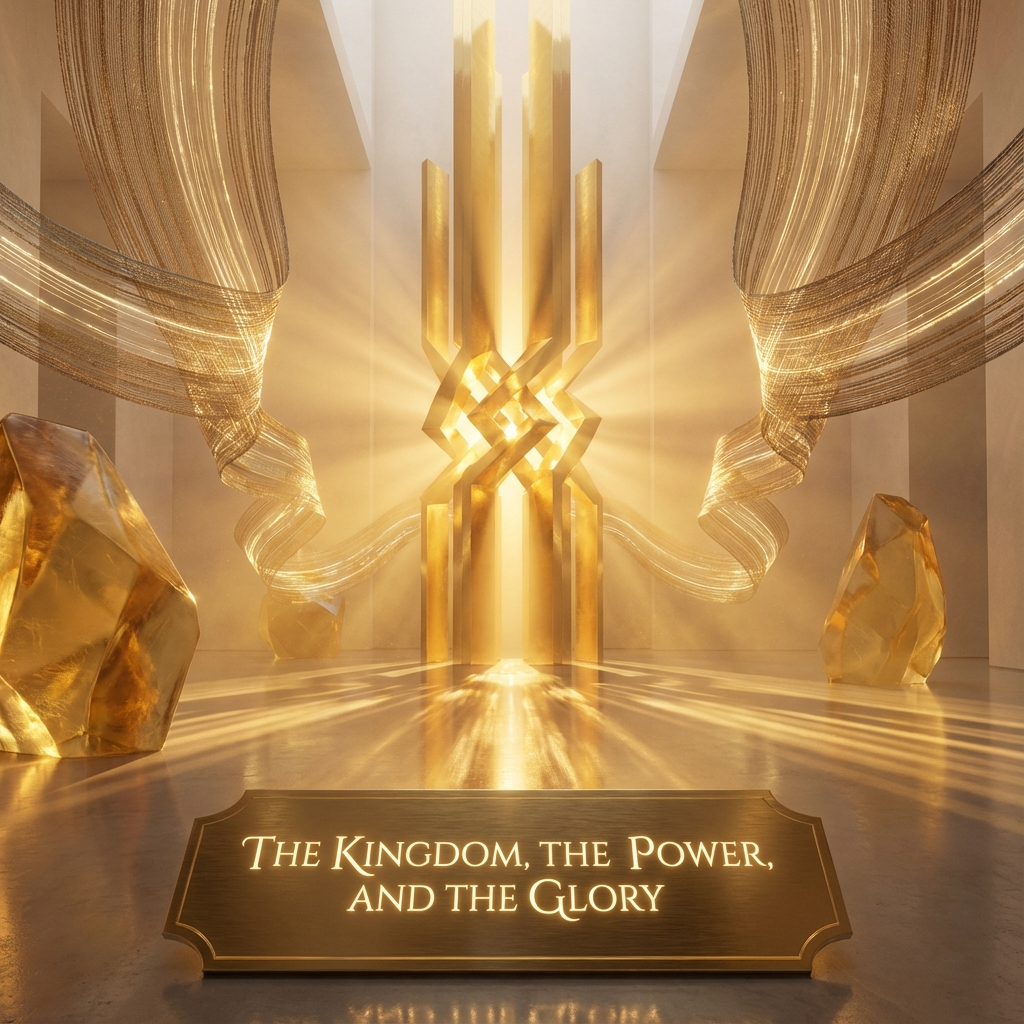
\includegraphics[width=0.75\textwidth,cfbox=gray!60 0.6pt 4pt]{kingdom_power.png}\\
\vspace{4pt}
{\small\itshape El Reino, el Poder y la Gloria: la resonancia eterna.}
\end{center}

\vspace{0.6cm}
El viaje llegaba a su fin. Estábamos sentados en un banco de la Plaza de Oriente, frente al Palacio Real.
—Tuyo es el Reino, el Poder y la Gloria —dijo Jesús, mirando el imponente edificio—. Pero no ese reino de piedras y guardias.

—¿Cuál entonces?

—El Reino es tu paz interior. El Poder es tu capacidad de elegir tu vibración en cada momento, pase lo que pase fuera. Y la Gloria... la Gloria es la alegría de ser quien eres. De ser un hijo del Universo.

Se levantó y estiró los brazos, como abrazando el mundo.
—No busques el poder fuera. No busques que te aplaudan. El verdadero poder es silencioso. Es la certeza de que nunca estás solo, de que la Vida te sostiene. Cuando entiendes eso, cuando lo sientes en tus células, ya estás en el Reino. Aquí y ahora. Entre Madrid, Las Rozas y Colmenarejo. El Reino está donde tú estás, si tú estás despierto.

Me miró con una intensidad que me atravesó el alma.
—No olvides esto, Francisco. Tienes el poder. Úsalo para vibrar alto. Úsalo para iluminar tu rincón del mundo. Esa es tu única tarea.